\section{Flight Dynamics}
Describing the flight dynamics of the quadcopter is done relative to an inertial reference frame. The flight velocities and the pitch,yaw and roll angles is described relative to the inertial frame. This frame is called the body frame. Common quadcopter use sensors like GPS, IMU etc. to keep track of the inertial frame. Since we are using the Qualisys motioncapture system at KIC, it will keep track of both the inertial frame and the body frame, so we will probably don't need to use sensors to keep track of the intertial and body frames. The qualisys system will 

\begin{figure}[H]
    \centering
    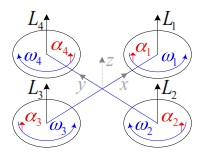
\includegraphics[width = 0.3\textwidth]{VAPIQ-PICTURES/Quadcopter.jpg}
    \caption{PICTURE caption}
    \label{fig:quadDynamics}
\end{figure}

Figure \ref{fig:quadDynamics} shows the control inputs of a variable pitch quadcopter. $\alpha_j$ represents the propeller pitch angle. $\omega_j$ represents the rotational speed of the propeller, while $L_j$ represents the lift force given from the propellers.\\ \\
$\phi$,$\theta$,$\psi$, denotes roll pitch and yaw of the quadcopter in the inertial frame. $v_x$, $v_y$, $v_y$, denotes the flight velocity's in the body frame.\\ 
The lift produced from the motors in the motor axis is described by $L_j$ = $b_L\alpha_j\omega_j^2$, where b_L is an aerodynamic constant.($b_L$ can be found bu using least-squares approximation). 